\documentclass{infufrgs}
\usepackage[utf8]{inputenc}
\usepackage{framed}
\usepackage{amsmath}
\usepackage{graphicx}
\usepackage{listings}
\usepackage{fancyvrb}
\usepackage{booktabs}
\usepackage{float}
\usepackage{multirow}
\usepackage{subcaption}

\graphicspath{{../../Selecao/analysis_output/figures/}}

% Configuração para snippets de código
\lstset{
    language=C++,
    basicstyle=\ttfamily\scriptsize,
    keywordstyle=\color{blue},
    stringstyle=\color{red},
    commentstyle=\color{green!50!black},
    numbers=left,
    numberstyle=\tiny\color{gray},
    stepnumber=1,
    numbersep=5pt,
    backgroundcolor=\color{gray!5},
    showspaces=false,
    showstringspaces=false,
    frame=single,
    rulecolor=\color{black!30},
    breaklines=true,
    breakatwhitespace=true,
    tabsize=2
}

\colorlet{shadecolor}{orange!15}

\title{Relatório de Análise Experimental: Seleção do $k$-ésimo Elemento}
\author{Rodrigues}{Juliana}

\begin{document}

\maketitle

\chapter{Relatório do Experimento}

%==================================================
\section{Introdução}
%==================================================

Este relatório descreve a avaliação empírica de três algoritmos para a \textbf{seleção do $k$-ésimo menor elemento} de um vetor não ordenado: a \textbf{Seleção Ingênua} (\texttt{NaiveSelection}: copia, ordena e indexa), o \textbf{Quickselect Aleatorizado} (\texttt{RandomizedQuickSelect}: pivô sorteado, partição, recursão) e a \textbf{Mediana das Medianas} (\texttt{MedianOfMediansSelection}: pivô determinístico via mediana das medianas de grupos de tamanho $g$, partição, recursão).

O objetivo central é determinar \emph{qual algoritmo é preferível na prática} e, quando não há vencedor absoluto, identificar os pontos de cruzamento de desempenho. A análise verifica as complexidades assintóticas teóricas por contagem de operações, traduz essas assíntotas em constantes reais de tempo, caracteriza a distribuição estatística do tempo do Quickselect, investiga a dependência em relação ao posto $k$ procurado, mede o efeito do tamanho de grupo $g$ da mediana das medianas (incluindo a atenção especial requerida ao caso $g = 3$) e investiga o que a biblioteca padrão (\texttt{std::nth\_element}) realmente implementa.

Todas as conclusões reportam o que os dados de fato mostram. Um achado central, discutido na Seção~\ref{sec:e7}, é que a mediana das medianas com partição de Lomuto \emph{não preserva} sua garantia linear sob entradas com muitas chaves repetidas, um resultado que motiva diretamente a investigação do \texttt{std::nth\_element}.

%==================================================
\section{Instâncias de Teste e Plano de Experimentos}
%==================================================

\subsection{Geradores de Instâncias}

Cada instância é um vetor de inteiros gerado de forma determinística a partir da tripla (tamanho $n$, distribuição, semente), de modo que \emph{a mesma instância é reproduzida identicamente} para todos os algoritmos comparados em uma célula, requisito de comparação justa. Apenas a aleatoriedade interna do Quickselect (semente do gerador de pivô) varia de forma independente. As nove distribuições implementadas estão na Tabela~\ref{tab:geradores}.

\begin{table}[H]
\centering
\caption{Catálogo de geradores de instâncias.}
\label{tab:geradores}
\begin{tabular}{lll}
\toprule
\textbf{ID} & \textbf{Descrição} & \textbf{Estressa} \\
\midrule
\texttt{uni}           & $n$ valores distintos, permutação aleatória   & caso médio (baseline) \\
\texttt{gaussian}      & valores $\sim \mathcal{N}(0,1)$ escalonados    & realismo \\
\texttt{alleq}         & todos os elementos iguais                      & partição de Lomuto \\
\texttt{dup\_2}        & apenas 2 valores distintos                     & baixa cardinalidade \\
\texttt{dup\_5}        & apenas 5 valores distintos                     & baixa cardinalidade \\
\texttt{sorted\_asc}   & já ordenado crescente                          & ordem adversária \\
\texttt{sorted\_desc}  & já ordenado decrescente                        & ordem adversária \\
\texttt{organpipe}     & crescente depois decrescente (``tubo de órgão'') & armadilha de mediana-de-3 \\
\texttt{nearly\_sorted}& ordenado + 1\% de trocas aleatórias            & quase ordenado \\
\bottomrule
\end{tabular}
\end{table}

O gerador \texttt{uni} produz uma \emph{permutação aleatória} de $\{0,\dots,n-1\}$ (valores distintos): como as contagens de comparação dependem apenas da ordem relativa, isso satisfaz a hipótese de chaves distintas usada no ajuste teórico do experimento E4. Uma distribuição desconhecida faz o gerador lançar exceção (em vez de substituir silenciosamente por uniforme), evitando rotular dados incorretamente.

\subsection{Plano de Experimentos}

Os experimentos são organizados em nove grupos (E1 a E9), cada um com objetivo, variável independente e métrica fixos (Tabela~\ref{tab:experimentos}). Os experimentos de \emph{contagem} (E1, E4, E7) são determinísticos quanto às operações e podem ser executados em paralelo; os de \emph{tempo} (E2, E3, E5, E6) são executados sequencialmente em um único núcleo, com o binário compilado em modo \emph{release} (sem \emph{AddressSanitizer}), para não enviesar os tempos absolutos.

\begin{table}[H]
\centering
\caption{Resumo dos experimentos realizados. $k$ medular $=\lfloor n/2 \rfloor$ salvo indicação contrária.}
\label{tab:experimentos}
\begin{tabular}{llll}
\toprule
\textbf{Teste} & \textbf{Objetivo} & \textbf{$n$ / variação} & \textbf{Reps.} \\
\midrule
E1 & Contagens (comparações, acessos) vs.\ $n$ & $10^2$ a $5{\times}10^5$ & 10 sementes \\
E2 & Tempo $T(n)$ + ajuste de regressão        & $5{\times}10^3$ a $2{,}5{\times}10^5$ & 30 \\
E3 & Distribuição de $T$ do Quickselect ($n$ fixo) & $10^3$, $10^4$, $10^5$ & 500 \\
E4 & Dependência do posto $k$                  & $k/n$ varrido ($n{=}10^4,10^5$) & 5 \\
E5 & Varredura de tamanho de grupo $g$         & $g \in \{3,5,7,9,11,15,21\}$ & 30 \\
E6 & Anomalia $g = 3$                          & $10^3$ a $10^6$, $g\in\{3,5,7\}$ & 8 \\
E7 & Robustez / entradas adversárias          & 9 distrib.\ $\times\ n$ até $4000$ & 3 \\
E8 & Estudo de cruzamento prático             & reusa E2 & n/a \\
E9 & Investigação do \texttt{std::nth\_element} & reusa E7 + E2 & n/a \\
\bottomrule
\end{tabular}
\end{table}

\subsection{Esquema do Arquivo CSV}

Cada execução do binário \texttt{run\_experiments} anexa uma linha em formato \emph{longo} a \texttt{data/benchmark\_data.csv} (uma linha por ensaio), e ao final uma cópia datada (\texttt{benchmark\_data\_\textit{AAAAMMDDThhmmss}.csv}) é arquivada. As colunas relevantes são:

\begin{center}
\texttt{experiment\_id, algorithm, n, k, k\_frac, g, distribution, instance\_seed,}\\
\texttt{comparisons, accesses, recursion\_depth, time\_ns, build, oracle\_match, timestamp}
\end{center}

As colunas \texttt{accesses} e \texttt{recursion\_depth} ficam vazias quando não fazem sentido (acessos não são instrumentáveis no \texttt{std::nth\_element}; profundidade só é registrada para Quickselect e mediana das medianas). A coluna \texttt{oracle\_match} registra a verificação de correção descrita adiante.

\subsection{Protocolo de Medição e Salvaguardas}

\textbf{Correção (oráculo).} Antes de registrar qualquer métrica, o resultado do algoritmo sob teste é comparado ao da \texttt{NaiveSelection} sobre a \emph{mesma} instância. Em todas as 3\,663 linhas geradas, \texttt{oracle\_match} foi verdadeiro, nenhuma divergência.

\textbf{Tempo.} Mede-se com \texttt{std::chrono::steady\_clock} (monotônico); reporta-se a \emph{mediana} de múltiplas repetições, robusta a \emph{jitter} de escalonamento. Como cada ensaio é um processo independente, o aquecimento de cache entre ensaios é irrelevante; a mediana cumpre o papel da medição robusta.

\textbf{Salvaguarda de tempo limite.} Cada célula tem um \emph{timeout} de 20\,s. Células degeneradas (Quickselect ou mediana das medianas sobre \texttt{alleq}) podem explodir para comportamento quadrático ou pior; ao estourar o limite, a célula simplesmente não gera linha, e a análise tolera a célula ausente.

\subsection{Ambiente de Execução}

Todos os experimentos foram executados na máquina descrita na Tabela~\ref{tab:ambiente}.

\begin{table}[H]
\centering
\caption{Configuração do ambiente de execução.}
\label{tab:ambiente}
\begin{tabular}{ll}
\toprule
\textbf{Componente} & \textbf{Especificação} \\
\midrule
Processador   & Intel Core Ultra 5 236V, 8 núcleos, 1 thread/núcleo, até 4{,}7\,GHz \\
Cache L1      & 320\,KiB dados + 512\,KiB instruções (8 instâncias) \\
Cache L2      & 14\,MiB (5 instâncias) \\
Cache L3      & 8\,MiB (1 instância) \\
Memória RAM   & 16\,GiB \\
Sistema operacional & Ubuntu 24.04.4 LTS, kernel 6.17.0-35-generic \\
Compilador    & g++ 13.3.0 (Ubuntu 13.3.0-6ubuntu2\textasciitilde24.04.1) \\
Flags (release) & \texttt{-std=c++17 -O3 -DNDEBUG} \\
\bottomrule
\end{tabular}
\end{table}

Os processos concorrentes do sistema operacional não foram controlados explicitamente; os tempos reportados correspondem à mediana de repetições independentes, atenuando interferências pontuais.

%==================================================
\section{Algoritmos e Análise de Complexidade}
%==================================================

\subsection{Seleção Ingênua}

A \texttt{NaiveSelection} copia o vetor (passagem por valor), ordena com \texttt{std::sort} e indexa a posição $k$:

\begin{lstlisting}[caption={Núcleo de NaiveSelection.h}]
T select(std::vector<T> data, int k, MetricsContext& metrics) override {
    std::sort(data.begin(), data.end(), [&metrics](const T& a, const T& b) {
        metrics.comparisons++;
        return a < b;
    });
    metrics.accesses++;
    return data[k];
}
\end{lstlisting}

\textbf{Complexidade:} a cópia é $O(n)$, a ordenação introsort da biblioteca é $\Theta(n \log n)$ comparações e a indexação é $O(1)$. Total: $\Theta(n \log n)$, \emph{independente de $k$}. Os acessos ao vetor não são instrumentados (ocorrem dentro do \texttt{std::sort}).

\subsection{Quickselect Aleatorizado}

O \texttt{RandomizedQuickSelect} sorteia um pivô uniformemente, particiona (esquema de Lomuto) e recorre apenas no lado que contém o posto $k$:

\begin{lstlisting}[caption={Partição de Lomuto e recursão (RandomizedQuickSelect.h)}]
int partition(std::vector<T>& data, int left, int right, int pivotIndex, MetricsContext& metrics) {
    T pivotValue = data[pivotIndex];
    metrics.accesses++;
    std::swap(data[pivotIndex], data[right]);   metrics.accesses += 4;
    int storeIndex = left;
    for (int i = left; i < right; i++) {
        metrics.comparisons++;  metrics.accesses++;
        if (data[i] < pivotValue) {
            std::swap(data[storeIndex], data[i]);  metrics.accesses += 4;
            storeIndex++;
        }
    }
    std::swap(data[right], data[storeIndex]);   metrics.accesses += 4;
    return storeIndex;
}
// ... na recursao:
std::uniform_int_distribution<int> dist(left, right);
int pivotIndex = partition(data, left, right, dist(rng), metrics);
if      (k == pivotIndex) return data[k];
else if (k <  pivotIndex) return quickSelect(data, left, pivotIndex - 1, k, metrics, depth + 1);
else                      return quickSelect(data, pivotIndex + 1, right, k, metrics, depth + 1);
\end{lstlisting}

\textbf{Complexidade:} o pivô aleatório dá, em valor esperado, partições suficientemente equilibradas, resultando em $O(n)$ comparações esperadas (a recorrência $T(n) = T(n/2) + O(n)$ no caso típico soma uma série geométrica $2n$). No \emph{pior caso} (pivôs sistematicamente ruins, ou todos os elementos iguais, ver E7), degrada para $\Theta(n^2)$. A partição de Lomuto envia os elementos \emph{iguais} ao pivô para o mesmo lado, o que é a raiz da degradação em \texttt{alleq}.

\subsection{Mediana das Medianas}

A \texttt{MedianOfMediansSelection} escolhe um pivô determinístico: divide o segmento em grupos de tamanho $g$, ordena cada grupo para obter sua mediana, e recorre sobre o vetor de medianas para achar a mediana das medianas:

\begin{lstlisting}[caption={Seleção do pivô determinístico (MedianOfMedians.h)}]
T get_pivot(std::vector<T>& data, int left, int right, MetricsContext& metrics, int depth = 1) {
    int n = right - left + 1;
    std::vector<T> medians;
    for (int i = 0; i < n; i += g) {
        int subRight = std::min(left + i + g - 1, right);
        medians.push_back(get_median_of_small_group(data, left + i, subRight, metrics));
    }
    return momSelect(medians, 0, medians.size() - 1, medians.size() / 2, metrics, depth + 1);
}
\end{lstlisting}

Em seguida, particiona em torno do pivô (também por Lomuto) e recorre no lado relevante.

\textbf{Complexidade (teórica):} para $g$ ímpar, a mediana das medianas garante que pelo menos $\approx n(g+1)/(4g)$ elementos ficam de cada lado, logo o lado maior tem no máximo $\approx n(3g-1)/(4g)$ elementos; o subproblema das medianas tem $n/g$ elementos. A recorrência $T(n) \le T(n/g) + T\!\big(\tfrac{3g-1}{4g}n\big) + O(n)$ \emph{contrai} (é linear) se e somente se $\tfrac{1}{g} + \tfrac{3g-1}{4g} < 1$, i.e.\ $g \ge 5$. Para $g = 3$ a soma é exatamente $1$, sem garantia de linearidade (ver E6). Assim, no papel, a mediana das medianas é $\Theta(n)$ de pior caso para $g \ge 5$.

\textbf{Ressalva de implementação (importante):} essa garantia linear pressupõe partição que trate corretamente elementos \emph{iguais} ao pivô. A partição de Lomuto de duas vias usada aqui não o faz: sob \texttt{alleq}, cada nível elimina apenas um elemento, e a recursão aninhada de \texttt{get\_pivot} faz o custo explodir para muito além de $\Theta(n^2)$ (Seção~\ref{sec:e7}). Optou-se por \emph{reportar} esse comportamento como achado, em vez de mascará-lo com uma partição de três vias.

\subsection{Biblioteca Padrão: \texttt{std::nth\_element}}

A \texttt{std::nth\_element} (libstdc++) implementa \textbf{introselect}: um Quickselect com pivô por mediana-de-3 que monitora a profundidade de recursão e, ao ultrapassar um limiar $\approx 2\log_2 n$, recua para um método de pior caso garantido (\emph{heapselect}). Assim evita simultaneamente o $\Theta(n^2)$ do Quickselect puro e o alto fator constante da mediana das medianas no caso comum. As comparações são instrumentáveis via comparador customizado (um \emph{lambda} que incrementa o contador); os acessos/trocas internos não o são, e isso é documentado como limitação.

\subsection{Resumo Teórico}

\begin{table}[H]
\centering
\caption{Complexidades teóricas (comparações) dos algoritmos.}
\label{tab:complexidades}
\begin{tabular}{lll}
\toprule
\textbf{Algoritmo} & \textbf{Complexidade} & \textbf{Observação} \\
\midrule
Seleção Ingênua          & $\Theta(n \log n)$                    & independente de $k$ \\
Quickselect Aleatorizado & $O(n)$ esperado / $\Theta(n^2)$ pior  & pior caso em chaves iguais \\
Mediana das Medianas ($g\ge 5$) & $\Theta(n)$ pior caso$^\ast$   & $^\ast$exige partição que trate duplicatas \\
Mediana das Medianas ($g = 3$)  & sem garantia linear           & $\tfrac1g + \tfrac{3g-1}{4g} = 1$ \\
\texttt{std::nth\_element} (introselect) & $O(n)$ pior caso     & Quickselect + recuo p/ heapselect \\
\bottomrule
\end{tabular}
\end{table}

%==================================================
\section{Resultados Experimentais e Análise}
%==================================================

\subsection{E1: Contagens de Operações vs.\ $n$}

O teste E1 mede comparações e acessos ao vetor em função de $n$ (instâncias \texttt{uni}, $k$ medular, $g = 5$, média de 10 sementes). A Tabela~\ref{tab:e1-exponents} traz os expoentes de crescimento ajustados por regressão log-log, e a Figura~\ref{fig:e1} mostra as curvas de comparações.

\begin{table}[H]
\centering
\caption{Expoentes empíricos de crescimento (E1, ajuste $k$ em $n^k$).}
\label{tab:e1-exponents}
\begin{tabular}{llrr}
\toprule
Algoritmo & Métrica & $k_\text{emp}$ & $R^2$ \\
\midrule
Seleção Ingênua          & comparações & 1{,}123 & 0{,}9997 \\
Quickselect              & comparações & 0{,}995 & 0{,}9968 \\
Mediana das Medianas     & comparações & 1{,}038 & 0{,}9996 \\
Quickselect              & acessos     & 0{,}984 & 0{,}9975 \\
Mediana das Medianas     & acessos     & 1{,}030 & 0{,}9998 \\
\midrule
Quickselect              & acessos/comparações (razão) & \multicolumn{2}{c}{3{,}10} \\
Mediana das Medianas     & acessos/comparações (razão) & \multicolumn{2}{c}{1{,}14} \\
\bottomrule
\end{tabular}
\end{table}

\begin{figure}[htbp]
    \centering
    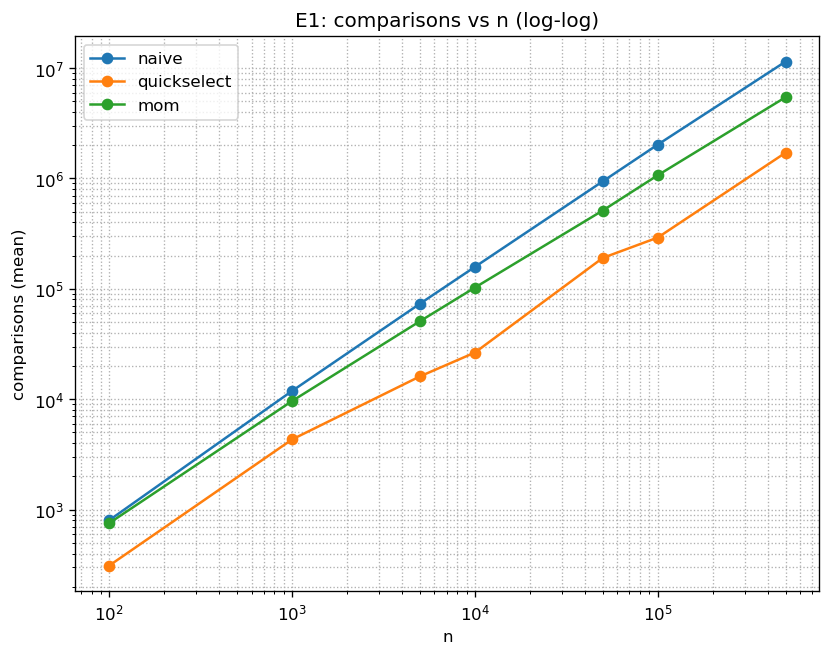
\includegraphics[width=0.70\textwidth]{e1_comparisons_vs_n.png}
    \caption{Comparações médias vs.\ $n$ em escala log-log (E1). A Seleção Ingênua ($k_\text{emp}=1{,}12$) cresce como $n\log n$; Quickselect ($0{,}99$) e Mediana das Medianas ($1{,}04$) são essencialmente lineares.}
    \label{fig:e1}
\end{figure}

Os expoentes confirmam as classes teóricas: a Seleção Ingênua tem expoente $1{,}12$ (acima de $1$, refletindo o fator $\log n$), enquanto Quickselect ($0{,}99$) e Mediana das Medianas ($1{,}04$) são lineares. Em números absolutos, a $n = 5{\times}10^5$ a Seleção Ingênua faz $\approx 11{,}4$ milhões de comparações, contra $5{,}4$ milhões da Mediana das Medianas e apenas $1{,}7$ milhão do Quickselect. A razão acessos/comparações $\approx 3{,}1$ do Quickselect é a assinatura da partição de Lomuto (cada troca custa 4 acessos extras), coerente com a faixa $3$ a $4$ esperada; a Mediana das Medianas, que faz menos trocas relativas, tem razão $\approx 1{,}1$.

\subsection{E2: Tempo de Parede e Ajuste de Regressão}

O teste E2 mede $T(n)$ no \emph{release} e ajusta três modelos candidatos ($a n + b$, $a\,n\ln n + b$, $a n^2 + b$) por mínimos quadrados, selecionando o de maior $R^2$ (Tabela~\ref{tab:e2-models}). A Figura~\ref{fig:e2} sobrepõe os dados e as curvas ajustadas.

\begin{table}[H]
\centering
\caption{Modelos de tempo: melhor ajuste por algoritmo (E2). $a$ em ns/unidade do modelo.}
\label{tab:e2-models}
\begin{tabular}{llrrc}
\toprule
Algoritmo & Melhor modelo & $a$ & $b$ (ns) & $R^2$ \\
\midrule
Seleção Ingênua          & $a\,n\ln n + b$ & 4{,}71  & $-1{,}12{\times}10^5$ & 0{,}9980 \\
Quickselect              & $a\,n + b$      & 9{,}67  & $-1{,}03{\times}10^4$ & 0{,}9988 \\
Mediana das Medianas     & $a\,n + b$      & 25{,}65 & $+1{,}48{\times}10^5$ & 0{,}9954 \\
\texttt{std::nth\_element}& $a\,n + b$      & 8{,}70  & $+1{,}5{\times}10^2$  & 0{,}9979 \\
\bottomrule
\end{tabular}
\end{table}

\begin{table}[H]
\centering
\caption{Tempos medianos ($\mu$s) vs.\ $n$ (E2, 30 repetições).}
\label{tab:e2-times}
\begin{tabular}{rrrrr}
\toprule
$n$ & Ingênua & Quickselect & Med.\ Medianas & \texttt{nth\_element} \\
\midrule
5\,000   &   208{,}6 &  36{,}6 &  131{,}4 &  33{,}4 \\
10\,000  &   453{,}6 &  80{,}6 &  268{,}1 &  86{,}6 \\
25\,000  & 1\,238{,}5 & 189{,}0 &  792{,}2 & 171{,}7 \\
50\,000  & 2\,305{,}4 & 526{,}4 & 1\,716{,}0 & 452{,}8 \\
100\,000 & 4\,865{,}6 & 962{,}1 & 2\,781{,}2 & 932{,}4 \\
250\,000 & 14\,704{,}5 & 2\,400{,}3 & 6\,484{,}7 & 2\,150{,}5 \\
\bottomrule
\end{tabular}
\end{table}

\begin{figure}[htbp]
    \centering
    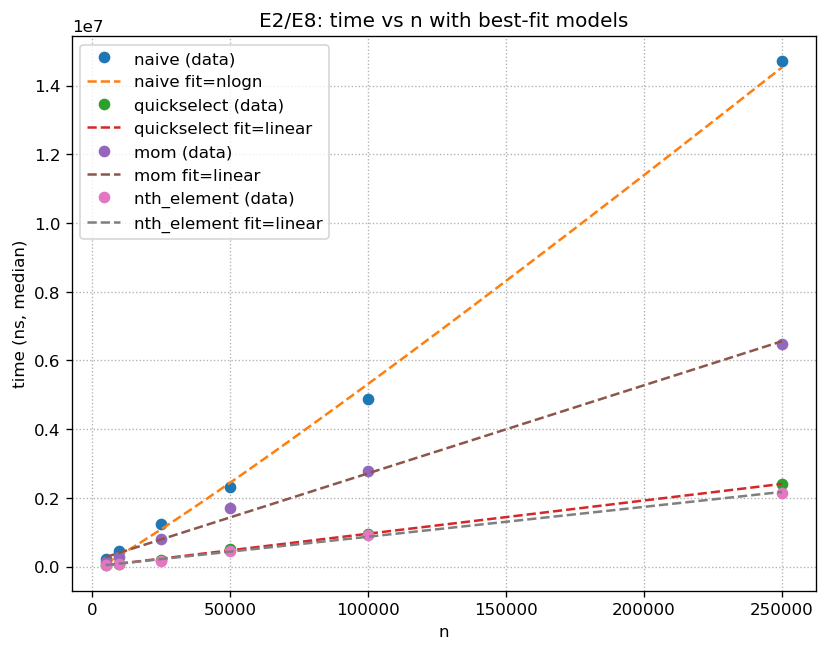
\includegraphics[width=0.72\textwidth]{e2_time_vs_n.png}
    \caption{Tempo mediano vs.\ $n$ com os melhores modelos ajustados (E2). A Seleção Ingênua é a única bem ajustada por $n\ln n$; as demais são lineares.}
    \label{fig:e2}
\end{figure}

O modelo $n\ln n$ vence para a Seleção Ingênua ($R^2 = 0{,}9980$ contra $0{,}9949$ do linear), enquanto Quickselect, Mediana das Medianas e \texttt{nth\_element} são melhor descritos por modelos \emph{lineares}. As constantes empíricas são o que de fato decide o vencedor prático dentro de uma mesma classe: $9{,}7$\,ns/elemento do Quickselect e $8{,}7$\,ns/elemento do \texttt{nth\_element} contra $25{,}7$\,ns/elemento da Mediana das Medianas, ou seja, a Mediana das Medianas é linear, mas com fator constante $\approx 2{,}7\times$ maior, fruto do custo de ordenar cada grupo e da recursão aninhada de medianas.

\subsection{E3: Distribuição do Tempo do Quickselect}

O teste E3 caracteriza $T$ (e as comparações) do Quickselect como variável aleatória, com $M = 500$ execuções independentes para $n \in \{10^3, 10^4, 10^5\}$. A Tabela~\ref{tab:e3} resume as estatísticas e a Figura~\ref{fig:e3} mostra os histogramas de comparações.

\begin{table}[H]
\centering
\caption{Estatísticas da distribuição de comparações do Quickselect (E3, $M=500$).}
\label{tab:e3}
\begin{tabular}{rrrrrr}
\toprule
$n$ & Média & Variância & Desvio & CV & Assimetria \\
\midrule
1\,000   &  3\,326   & $9{,}7{\times}10^5$  &    986 & 0{,}296 & 0{,}62 \\
10\,000  & 34\,031   & $9{,}9{\times}10^7$  & 9\,961 & 0{,}293 & 0{,}83 \\
100\,000 & 334\,120  & $8{,}4{\times}10^9$  & 91\,448 & 0{,}274 & 0{,}62 \\
\bottomrule
\end{tabular}
\end{table}

\begin{figure}[htbp]
    \centering
    \begin{subfigure}[t]{0.32\textwidth}
        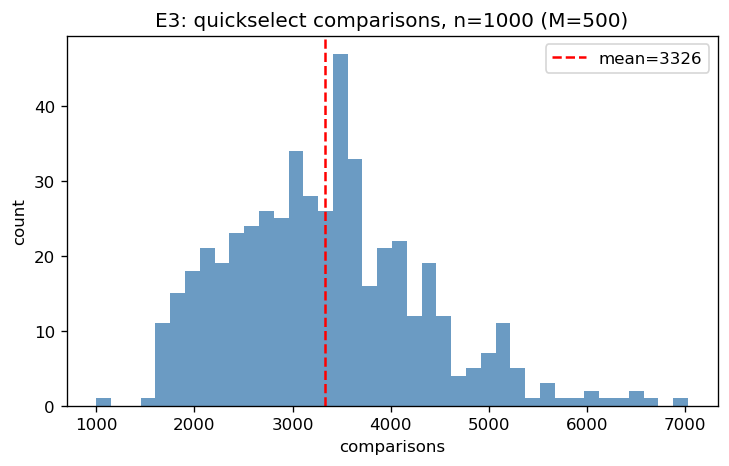
\includegraphics[width=\linewidth]{e3_hist_comparisons_n1000.png}
        \caption{$n = 10^3$}
    \end{subfigure}\hfill
    \begin{subfigure}[t]{0.32\textwidth}
        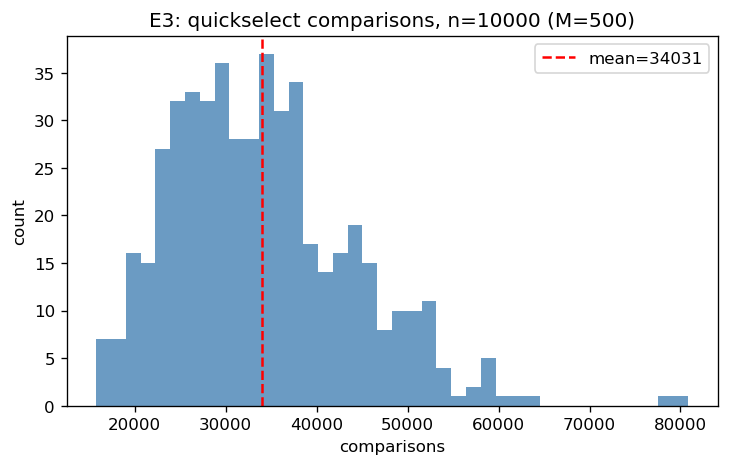
\includegraphics[width=\linewidth]{e3_hist_comparisons_n10000.png}
        \caption{$n = 10^4$}
    \end{subfigure}\hfill
    \begin{subfigure}[t]{0.32\textwidth}
        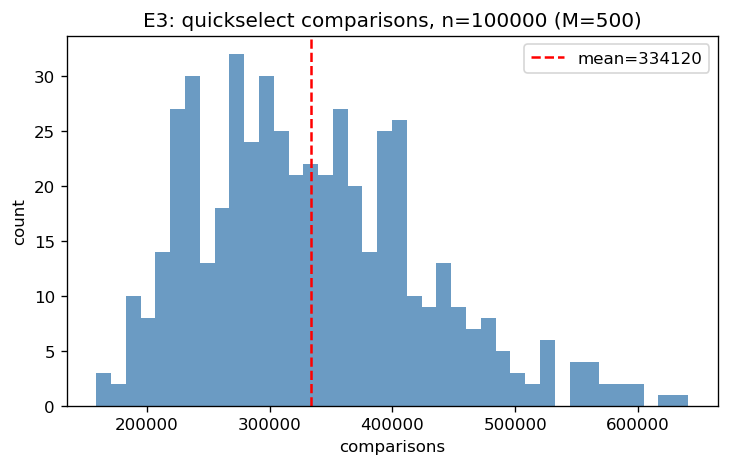
\includegraphics[width=\linewidth]{e3_hist_comparisons_n100000.png}
        \caption{$n = 10^5$}
    \end{subfigure}
    \caption{Histogramas de comparações do Quickselect (E3). A cauda à direita (assimetria positiva $\approx 0{,}6$ a $0{,}8$) reflete sequências ocasionais de pivôs infelizes; nenhum \emph{outlier} foi descartado.}
    \label{fig:e3}
\end{figure}

A média escala como $n^{1{,}00}$ e o desvio-padrão como $n^{0{,}98}$, logo a \textbf{variância escala como $n^{1{,}97} \approx n^2$}, exatamente a previsão teórica de que média e desvio crescem ambos linearmente em $n$. Como consequência, o coeficiente de variação CV $= \sigma/\mu$ permanece \emph{praticamente constante} ($\approx 0{,}27$ a $0{,}30$): a variabilidade relativa não cresce com a escala. As distribuições são moderadamente assimétricas à direita (assimetria $0{,}6$ a $0{,}8$), confirmando a presença de uma cauda de pivôs infelizes que, contudo, não se agrava em termos relativos com $n$.

\subsection{E4: Dependência do Posto $k$}

O teste E4 varre $k/n$ para $n \in \{10^4, 10^5\}$ (Figura~\ref{fig:e4}, Tabela~\ref{tab:e4}). A Seleção Ingênua é, por construção, \emph{independente de $k$} (ordena tudo): $2{,}05$ milhões de comparações para qualquer $k$ a $n = 10^5$, um teste de sanidade que confirma o custo de ordenação total. A Mediana das Medianas é quase plana ($\approx 1{,}07$ milhão), graças à sua divisão garantida $\approx 30/70$ independentemente de $k$. O Quickselect mostra dependência \emph{moderada}: mais barato sobretudo no extremo superior ($\approx 182$\,mil em $k/n = 0{,}99$) e com um pico em postos interiores ($\approx 322$\,mil em $k/n = 0{,}75$). A forma é qualitativamente compatível com a curva esperada $2[n + k\ln(n/k) + (n-k)\ln(n/(n-k))]$, mas o efeito é modesto frente ao ruído e o pico empírico não cai exatamente na mediana prevista pela fórmula simétrica, ou seja, a corcova teórica é apenas \emph{sugerida}, não confirmada com nitidez.

\begin{table}[H]
\centering
\caption{Comparações médias vs.\ posto $k/n$ em $n = 10^5$ (E4).}
\label{tab:e4}
\begin{tabular}{rrrr}
\toprule
$k/n$ & Ingênua & Quickselect & Med.\ Medianas \\
\midrule
0{,}00 & 2\,047\,733 & 242\,418 & 1\,068\,956 \\
0{,}25 & 2\,047\,733 & 289\,708 & 1\,076\,239 \\
0{,}50 & 2\,047\,733 & 252\,335 & 1\,069\,369 \\
0{,}75 & 2\,047\,733 & 322\,211 & 1\,064\,423 \\
0{,}99 & 2\,047\,733 & 184\,203 & 1\,068\,170 \\
\bottomrule
\end{tabular}
\end{table}

\begin{figure}[htbp]
    \centering
    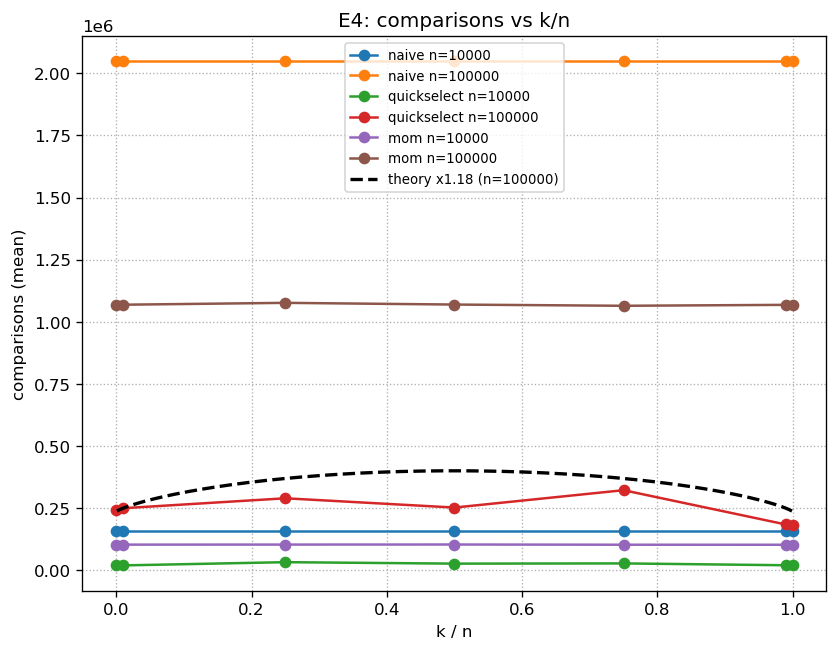
\includegraphics[width=0.72\textwidth]{e4_k_dependency.png}
    \caption{Comparações vs.\ $k/n$ (E4). Ingênua plana (independente de $k$); Mediana das Medianas quase plana; Quickselect com dependência moderada, mais barato nos extremos. A curva tracejada é o ajuste teórico do Quickselect.}
    \label{fig:e4}
\end{figure}

\subsection{E5: Tamanho de Grupo da Mediana das Medianas}

O teste E5 varia $g$ (instâncias \texttt{uni}, $n = 10^5$, $k$ medular) e analisa o efeito \emph{teórico e empírico}. A Tabela~\ref{tab:e5} reúne ambas as facetas: as métricas medidas (comparações, tempo, profundidade de recursão) e a teoria de poda por grupo.

\begin{table}[H]
\centering
\caption{Efeito do tamanho de grupo $g$ (E5): empírico (comparações, tempo mediano, profundidade) e teórico (fração do lado maior $\tfrac{3g-1}{4g}$ e soma da recorrência).}
\label{tab:e5}
\begin{tabular}{rrrrrc}
\toprule
$g$ & Comparações & Tempo ($\mu$s) & Prof.\ rec. & Frac.\ recursão & Linear? \\
\midrule
3  & 1\,420\,506 & 5\,567{,}8 & 16{,}4 & 0{,}667 & \textbf{não} (soma $=1{,}00$) \\
5  & 1\,080\,606 & 2\,728{,}9 & 15{,}6 & 0{,}700 & sim (0{,}90) \\
7  & \textbf{1\,053\,384} & 2\,397{,}8 & 15{,}0 & 0{,}714 & sim (0{,}86) \\
9  & 1\,120\,793 & \textbf{2\,229{,}2} & 14{,}7 & 0{,}722 & sim (0{,}83) \\
11 & 1\,177\,582 & 2\,727{,}5 & 14{,}6 & 0{,}727 & sim (0{,}82) \\
15 & 1\,325\,278 & 2\,495{,}4 & 14{,}3 & 0{,}733 & sim (0{,}80) \\
21 & 1\,483\,573 & 2\,835{,}2 & 13{,}7 & 0{,}738 & sim (0{,}79) \\
\bottomrule
\end{tabular}
\end{table}

\begin{figure}[htbp]
    \centering
    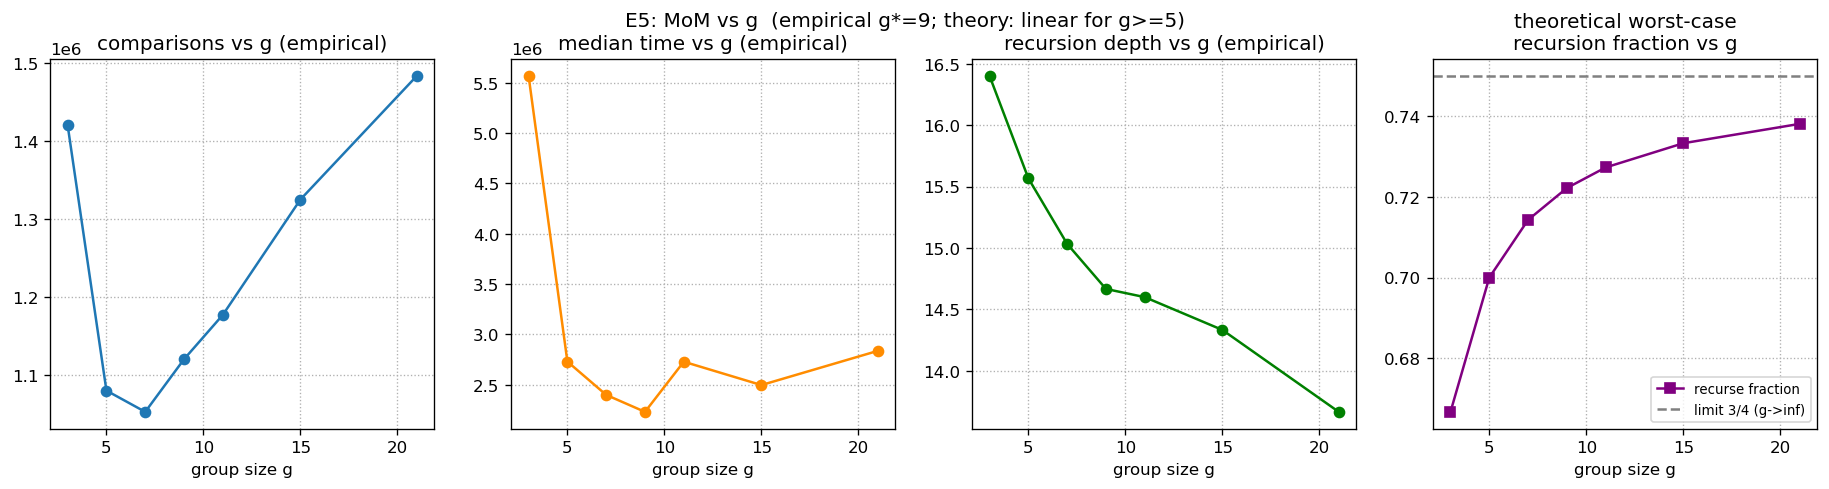
\includegraphics[width=\textwidth]{e5_group_size_sweep.png}
    \caption{Mediana das Medianas vs.\ $g$ (E5): comparações, tempo e profundidade de recursão (empíricos) e a fração teórica de recursão $\tfrac{3g-1}{4g}$ (que tende a $3/4$). A curva de comparações tem forma de U.}
    \label{fig:e5}
\end{figure}

O comportamento empírico tem a forma de \textbf{U} prevista: $g$ pequeno gera muitos níveis de recursão (mais comparações), enquanto $g$ grande encarece a mediana por grupo (a ordenação de cada grupo cresce com $g$). As comparações são minimizadas em $g = 7$ ($1{,}05$ milhão) e o tempo mediano em $g = 9$ ($2{,}23$\,ms); o $g = 5$ comumente citado é competitivo, mas não ótimo nesta máquina. A profundidade de recursão cai monotonicamente com $g$ (de $16{,}4$ em $g=3$ a $13{,}7$ em $g=21$): mais grupos por nível significam menos níveis, o que fornece a explicação mecanística da forma das outras curvas. A coluna teórica mostra a transição-chave: $g = 3$ tem soma de recorrência exatamente $1{,}00$ (sem garantia linear), e todo $g \ge 5$ contrai.

\subsection{E6: A Anomalia $g = 3$ (Atenção Especial)}

O teste E6 investiga por que $g = 3$ não é provadamente linear. A recorrência $T(n) \le T(n/3) + T(\tfrac{3\cdot 3-1}{4\cdot 3}n) + O(n) = T(n/3) + T(2n/3) + O(n)$ tem soma de frações $\tfrac13 + \tfrac23 = 1$: ela \emph{não contrai}, podendo derivar para $\Theta(n\log n)$ ou pior no \emph{pior caso}. Para quantificar empiricamente, varremos $n$ de $10^3$ a $10^6$ com $g \in \{3,5,7\}$ sobre \texttt{uni} e \texttt{sorted\_asc} (Tabela~\ref{tab:e6}, Figura~\ref{fig:e6}).

\begin{table}[H]
\centering
\caption{Expoentes empíricos de comparações vs.\ $n$ por $g$ (E6, até $n=10^6$).}
\label{tab:e6}
\begin{tabular}{llrr}
\toprule
Distribuição & $g$ & $k_\text{emp}$ & $R^2$ \\
\midrule
\texttt{uni}        & 3 & 1{,}038 & 0{,}9999 \\
\texttt{uni}        & 5 & 1{,}016 & 0{,}9999 \\
\texttt{uni}        & 7 & 1{,}016 & 0{,}9999 \\
\texttt{sorted\_asc}& 3 & 1{,}014 & 0{,}980 \\
\texttt{sorted\_asc}& 5 & 1{,}015 & 1{,}000 \\
\texttt{sorted\_asc}& 7 & 1{,}070 & 0{,}989 \\
\bottomrule
\end{tabular}
\end{table}

\begin{figure}[htbp]
    \centering
    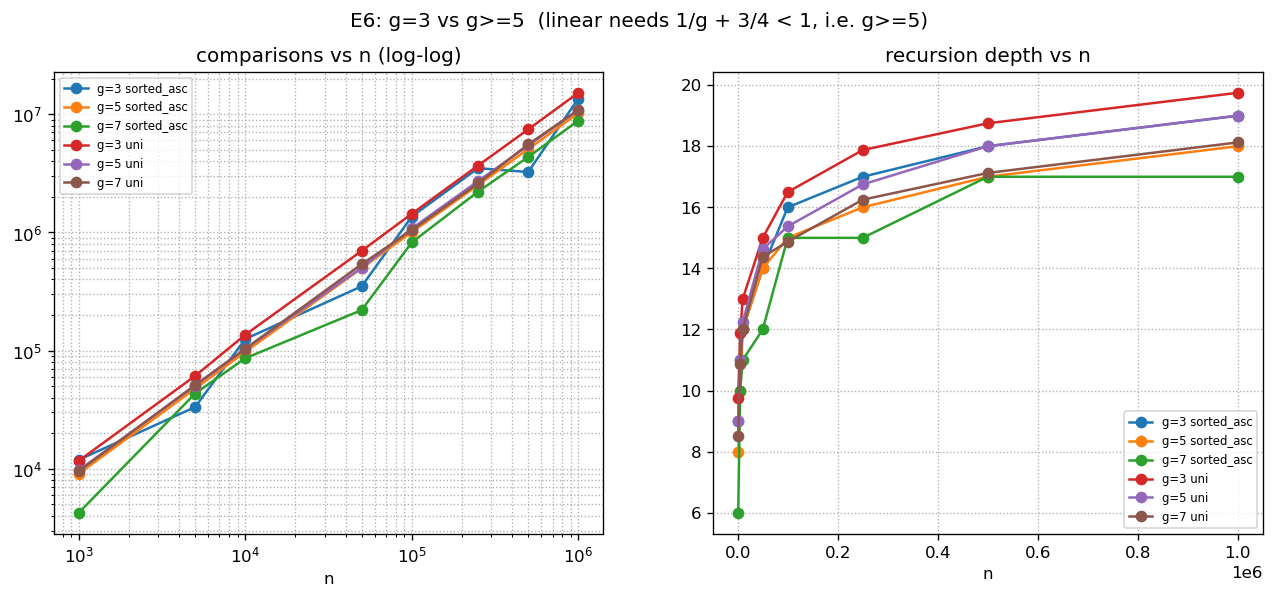
\includegraphics[width=\textwidth]{e6_g3_anomaly.png}
    \caption{Anomalia $g=3$ (E6): comparações vs.\ $n$ (log-log) e profundidade de recursão vs.\ $n$, para $g\in\{3,5,7\}$. Em entradas \texttt{uni}/\texttt{sorted}, $g=3$ não se separa visivelmente de $g\ge 5$ mesmo a $n=10^6$.}
    \label{fig:e6}
\end{figure}

\textbf{Em entradas uniformes e ordenadas, $g = 3$ permanece linear} mesmo a $n = 10^6$ ($k_\text{emp} = 1{,}04$ em \texttt{uni}, indistinguível dos $1{,}02$ de $g = 5/7$). A degradação de $g = 3$ é um fenômeno de \emph{pior caso}: a recorrência não contrair é uma cota estrutural, mas em dados benignos a mediana das medianas escolhe pivôs muito melhores que a garantia $\tfrac13$, produzindo divisões quase equilibradas e, portanto, tempo linear. A profundidade de recursão de $g = 3$ é apenas ligeiramente superior à de $g \ge 5$ ($16{,}4$ vs.\ $15{,}6$ em $n=10^5$, Tabela~\ref{tab:e5}). A recomendação prática que decorre é a mesma adotada pelo introselect: usar $g \ge 5$ (ou um recuo híbrido) para \emph{garantir} a linearidade, já que a ausência de garantia em $g = 3$ poderia ser explorada por uma entrada adversária construída para tanto.

\subsection{E7: Robustez e Estresse com Duplicatas}
\label{sec:e7}

O teste E7 submete os algoritmos às famílias adversárias e de baixa cardinalidade (Tabela~\ref{tab:e7}, Figuras~\ref{fig:e7} e~\ref{fig:e7deg}). 
\begin{table}[H]
\centering
\caption{Comparações médias por distribuição em $n = 4000$ (E7). Em negrito, as explosões super-lineares.}
\label{tab:e7}
\begin{tabular}{lrrrr}
\toprule
Distribuição & Ingênua & Quickselect & Med.\ Medianas & \texttt{nth\_element} \\
\midrule
\texttt{uni}          & 57\,280 &  11\,649 &  34\,007 & 11\,810 \\
\texttt{gaussian}     & 57\,374 &  12\,343 &  41\,034 & 10\,628 \\
\texttt{sorted\_asc}  & 54\,413 &  11\,548 &  38\,423 & 10\,018 \\
\texttt{organpipe}    & 113\,036 & 17\,038 &  33\,742 & 42\,203 \\
\texttt{dup\_5}       & 40\,666 & 251\,388 & \textbf{21\,041\,285} & 10\,306 \\
\texttt{dup\_2}       & 40\,562 & \textbf{745\,884} & \textbf{324\,989\,362} & 10\,748 \\
\texttt{alleq}        & 36\,939 & \textbf{6\,000\,999} & \emph{timeout} & 8\,035 \\
\bottomrule
\end{tabular}
\end{table}

\begin{figure}[htbp]
    \centering
    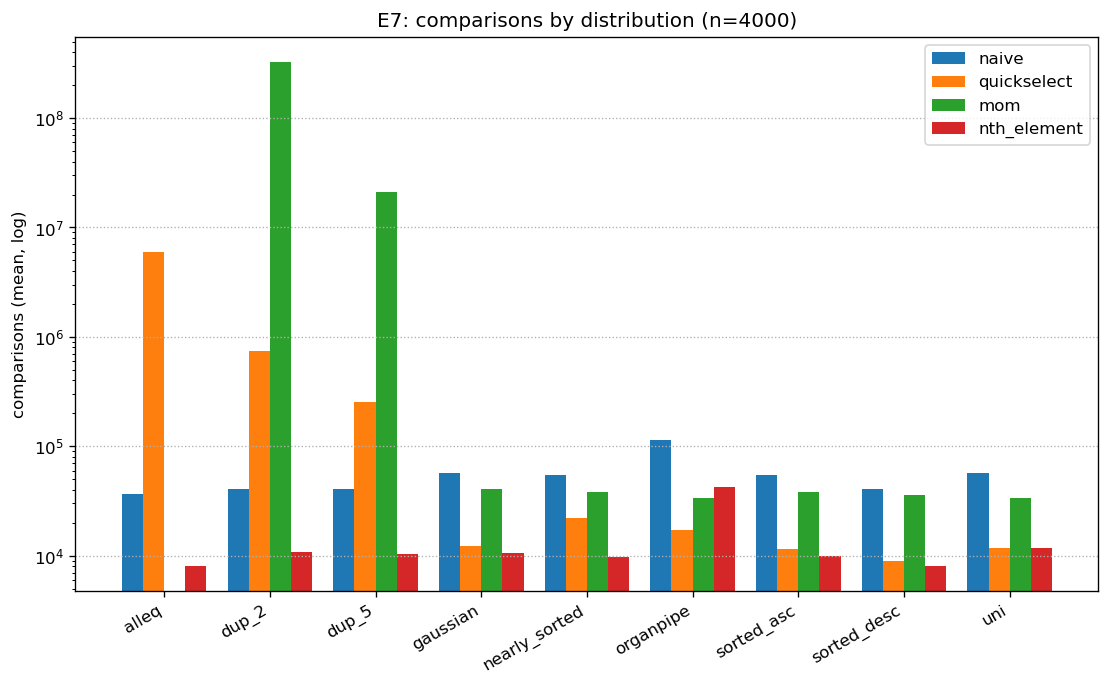
\includegraphics[width=0.80\textwidth]{e7_by_distribution.png}
    \caption{Comparações por distribuição em escala log (E7, $n=4000$). Quickselect e Mediana das Medianas explodem em entradas de baixa cardinalidade; Ingênua e \texttt{nth\_element} permanecem controlados.}
    \label{fig:e7}
\end{figure}

\begin{figure}[htbp]
    \centering
    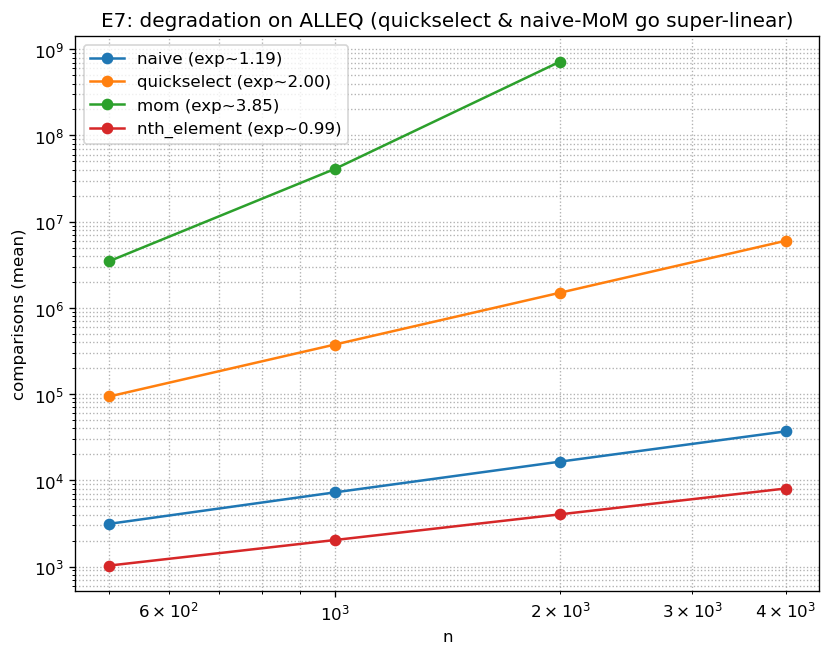
\includegraphics[width=0.66\textwidth]{e7_alleq_degradation.png}
    \caption{Degradação em \texttt{alleq}: comparações vs.\ $n$ (log-log). Os expoentes ajustados revelam a natureza de cada falha (Tabela~\ref{tab:e7deg}).}
    \label{fig:e7deg}
\end{figure}

\begin{table}[H]
\centering
\caption{Expoente de comparações vs.\ $n$ na entrada \texttt{alleq} (E7).}
\label{tab:e7deg}
\begin{tabular}{lrc}
\toprule
Algoritmo & $k_\text{emp}$ (\texttt{alleq}) & Diagnóstico \\
\midrule
Seleção Ingênua          & 1{,}19 & $n\log n$ (sem degradação) \\
\texttt{std::nth\_element}& 0{,}99 & linear (introselect resiste) \\
Quickselect              & 2{,}00 & \textbf{quadrático} (Lomuto + chaves iguais) \\
Mediana das Medianas     & 3{,}85 & \textbf{catastrófico} (recursão aninhada) \\
\bottomrule
\end{tabular}
\end{table}

Sob \texttt{alleq}, o Quickselect degrada para \emph{exatamente} $\Theta(n^2)$ (expoente $2{,}00$): com todos os elementos iguais, a partição de Lomuto envia tudo para um lado e cada nível remove apenas um elemento. O mesmo mecanismo, agravado pela recursão aninhada de \texttt{get\_pivot}, leva a Mediana das Medianas a um expoente $3{,}85$, pior que cúbico; a célula a $n = 4000$ sequer terminou dentro do \emph{timeout} de 20\,s. \textbf{A mediana das medianas com partição de Lomuto não preserva a garantia linear sob chaves repetidas}. A garantia de pior caso da literatura pressupõe uma partição que isole os elementos iguais ao pivô (partição de três vias); a implementação de duas vias aqui usada não o faz. As distribuições de \emph{ordem} adversária (\texttt{sorted}, \texttt{organpipe}) não derrubam o Quickselect, pois seu pivô é \emph{aleatório}, imune a arranjos fixos.

\subsection{E8: Estudo de Cruzamento Prático}

O teste E8 reusa os tempos de E2 (instâncias \texttt{uni}, $k$ medular) para responder qual algoritmo vence na prática. A Tabela~\ref{tab:e8} lista o mais rápido por $n$.

\begin{table}[H]
\centering
\caption{Algoritmo mais rápido por $n$ (E8, tempo mediano).}
\label{tab:e8}
\begin{tabular}{rll}
\toprule
$n$ & Mais rápido & Tempo ($\mu$s) \\
\midrule
5\,000   & \texttt{nth\_element} & 33{,}4 \\
10\,000  & quickselect           & 80{,}6 \\
25\,000  & \texttt{nth\_element} & 171{,}7 \\
50\,000  & \texttt{nth\_element} & 452{,}8 \\
100\,000 & \texttt{nth\_element} & 932{,}4 \\
250\,000 & \texttt{nth\_element} & 2\,150{,}5 \\
\bottomrule
\end{tabular}
\end{table}

Sob entrada uniforme \emph{não há um cruzamento limpo}: o Quickselect e o \texttt{std::nth\_element} são estatisticamente \textbf{empatados} (ambos lineares, com constantes $9{,}7$ e $8{,}7$\,ns/elemento), alternando a liderança dentro do ruído de medição, o ``cruzamento'' detectado entre $n = 5000$ e $25000$ é artefato de \emph{jitter}, não um regime real. Ambos dominam a Mediana das Medianas (linear, mas $\approx 2{,}7\times$ mais lenta) e a Seleção Ingênua ($n\log n$, a mais lenta em toda a faixa) em todos os $n$. O ordenamento prático é, portanto: \texttt{nth\_element} $\approx$ Quickselect $<$ Mediana das Medianas $<$ Ingênua. Conclui-se que, para entrada aleatória, \emph{o Quickselect domina a partir de $n$ pequeno e a Mediana das Medianas só é preferível sob as condições adversárias caracterizadas em E7, não por $n$ isoladamente}.

\subsection{E9: Investigação do \texttt{std::nth\_element} (Introselect)}

O teste E9 confronta o \texttt{std::nth\_element} aos três algoritmos sobre toda a suíte de E7 (Tabela~\ref{tab:e7}, Figura~\ref{fig:e9}). O resultado é a síntese de todo o relatório.

\begin{figure}[htbp]
    \centering
    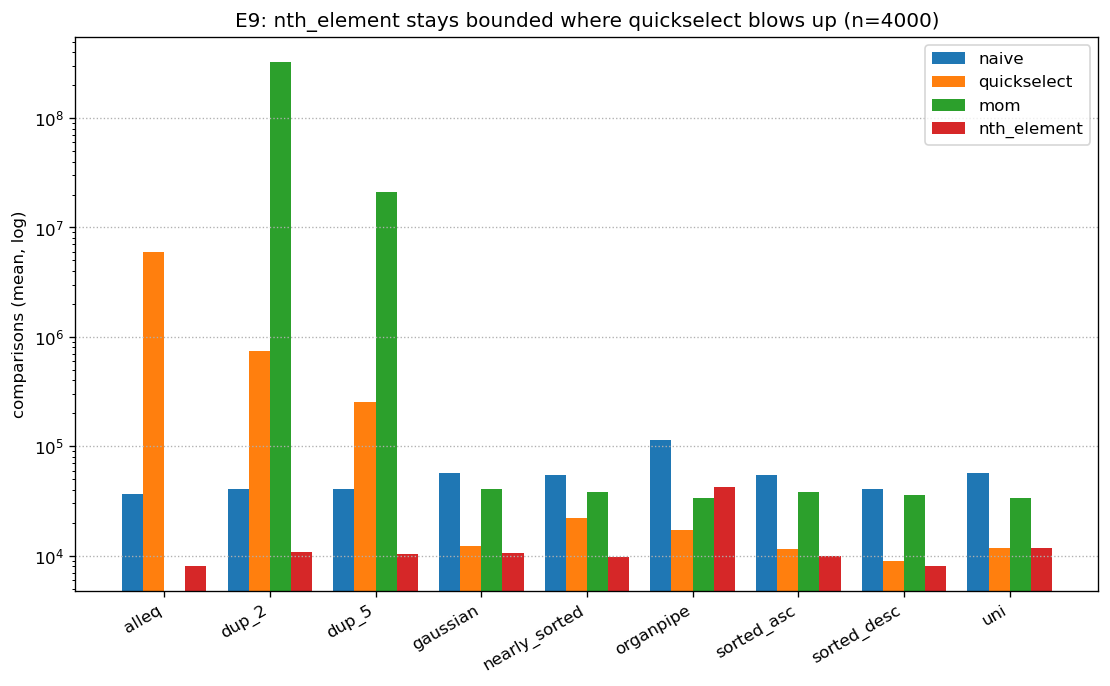
\includegraphics[width=0.80\textwidth]{e9_nth_element_vs_others.png}
    \caption{\texttt{std::nth\_element} vs.\ os três algoritmos na suíte adversária (E9, $n=4000$, escala log). O \texttt{nth\_element} mantém custo limitado onde o Quickselect \emph{e} a Mediana das Medianas explodem.}
    \label{fig:e9}
\end{figure}

O \texttt{std::nth\_element} permanece \textbf{limitado em $\approx 8$ a $12$ mil comparações ($\approx 2$ a $3n$) em \emph{todas} as distribuições}, incluindo \texttt{alleq} ($8{,}0$\,mil) e \texttt{dup\_2} ($10{,}7$\,mil), enquanto o Quickselect explode para $6$ milhões em \texttt{alleq} e a Mediana das Medianas para $325$ milhões em \texttt{dup\_2}. O introselect \emph{combina} a velocidade média do Quickselect em \texttt{uni} (E2: praticamente empatados) com uma robustez que \emph{nenhum} dos dois algoritmos puros possui, evita tanto o $\Theta(n^2)$ do Quickselect quanto a degradação por duplicatas da nossa mediana das medianas. Conclui-se que é por isso que a biblioteca padrão não usa nenhum dos três isoladamente: ela usa o Quickselect no caso comum, mas com mediana-de-3 e um \emph{recuo} para um método de pior caso garantido quando a profundidade de recursão denuncia uma sequência de pivôs ruins.

%==================================================
\section{Conclusão}
%==================================================

Os experimentos verificaram as complexidades teóricas e, mais importante, expuseram onde a teoria de livro-texto encontra ressalvas de implementação:

\textbf{Contagens e tempo (E1, E2).} A Seleção Ingênua é $\Theta(n\log n)$ (expoente $1{,}12$); Quickselect e Mediana das Medianas são lineares (expoentes $0{,}99$ e $1{,}04$). Em constantes de tempo, Quickselect ($9{,}7$\,ns/elem.) e \texttt{nth\_element} ($8{,}7$) batem a Mediana das Medianas ($25{,}7$) por fator $\approx 2{,}7\times$, apesar da mesma classe assintótica.

\textbf{Distribuição e posto (E3, E4).} O tempo do Quickselect tem média e desvio lineares em $n$ (variância $\sim n^2$, CV $\approx 0{,}28$ constante) com cauda direita suave. A Seleção Ingênua é independente de $k$; a Mediana das Medianas é quase plana; o Quickselect tem dependência moderada, mais barato nos extremos.

\textbf{Tamanho de grupo e $g = 3$ (E5, E6).} A curva de custo vs.\ $g$ tem forma de U, com ótimo empírico em $g = 7$ (comparações) a $g = 9$ (tempo). A teoria de poda ($\tfrac1g + \tfrac{3g-1}{4g} < 1 \Leftrightarrow g \ge 5$) coincide com a ausência de garantia em $g = 3$; empiricamente, porém, $g = 3$ permanece linear em entradas benignas até $n = 10^6$, a anomalia é estritamente de pior caso.

\textbf{Robustez e biblioteca padrão (E7, E9).} O achado mais forte: sob \texttt{alleq}/baixa cardinalidade, o Quickselect degrada para $\Theta(n^2)$ e a \emph{mediana das medianas com partição de Lomuto degrada ainda mais} (expoente $3{,}85$), pois a partição de duas vias não isola chaves iguais. O \texttt{std::nth\_element} (introselect) é o único a permanecer linear em toda a suíte, justificando empiricamente por que as bibliotecas reais não adotam nenhum dos três algoritmos puros.

\textbf{Recomendação prática (E8).} Para entrada aleatória, \emph{não há vencedor absoluto entre Quickselect e \texttt{std::nth\_element}}, ambos lineares e empatados, dominando a Mediana das Medianas e a Seleção Ingênua em toda a faixa. A Seleção Ingênua só se justifica quando o vetor ordenado também é necessário; a Mediana das Medianas, como garantia de pior caso \emph{desde que} sua partição trate duplicatas. Na ausência dessa correção, e no caso geral, o \texttt{std::nth\_element} é a escolha recomendada: tão rápido quanto o Quickselect no caso médio e imune às patologias que derrubam os algoritmos puros.

\end{document}
